\documentclass[tikz,border=8pt]{standalone}
\usepackage[T1]{fontenc}
\usepackage{helvet}
\renewcommand{\familydefault}{\sfdefault}
\usetikzlibrary{arrows.meta, backgrounds}

\definecolor{queryfill}{HTML}{DFF7F3}
\definecolor{queryborder}{HTML}{1BA99C}
\definecolor{corpusfill}{HTML}{FFF4D6}
\definecolor{corpusborder}{HTML}{D9A441}
\definecolor{bm25fill}{HTML}{FFE9C8}
\definecolor{bm25border}{HTML}{D88922}
\definecolor{llmfill}{HTML}{E9EDFF}
\definecolor{llmborder}{HTML}{6979C9}
\definecolor{nodefill}{HTML}{E8F2FF}
\definecolor{nodeborder}{HTML}{4E8CD8}
\definecolor{outfill}{HTML}{E7F6E7}
\definecolor{outborder}{HTML}{4FA64F}
\definecolor{softgray}{HTML}{F4F7FB}
\definecolor{darkline}{HTML}{333333}

\tikzset{
  card/.style={
    rectangle,
    rounded corners=5pt,
    align=center,
    draw=darkline,
    line width=0.8pt,
    minimum height=0.82cm,
    font=\small
  },
  query/.style={card, fill=queryfill, draw=queryborder, minimum width=2.05cm},
  corpus/.style={card, fill=corpusfill, draw=corpusborder, minimum width=2.25cm},
  bm25/.style={card, fill=bm25fill, draw=bm25border, minimum width=2.55cm, font=\small\bfseries},
  llm/.style={card, fill=llmfill, draw=llmborder, minimum width=2.7cm, font=\small\bfseries},
  output/.style={card, fill=outfill, draw=outborder, minimum width=2.7cm},
  artifact/.style={card, fill=white, minimum width=2.75cm},
  softbox/.style={rectangle, rounded corners=8pt, draw=darkline, fill=softgray, line width=0.7pt},
  doc/.style={rectangle, rounded corners=4pt, fill=corpusfill, draw=corpusborder, line width=0.7pt, minimum width=0.42cm, minimum height=0.58cm},
  node/.style={circle, fill=nodefill, draw=nodeborder, line width=0.7pt, minimum size=0.29cm},
  finalnode/.style={circle, fill=outfill, draw=outborder, line width=0.7pt, minimum size=0.29cm},
  phase/.style={font=\small\bfseries, align=center},
  flow/.style={-{Latex[length=2.2mm]}, line width=0.85pt, draw=darkline},
  faint/.style={dashed, darkline, opacity=0.32}
}

\begin{document}
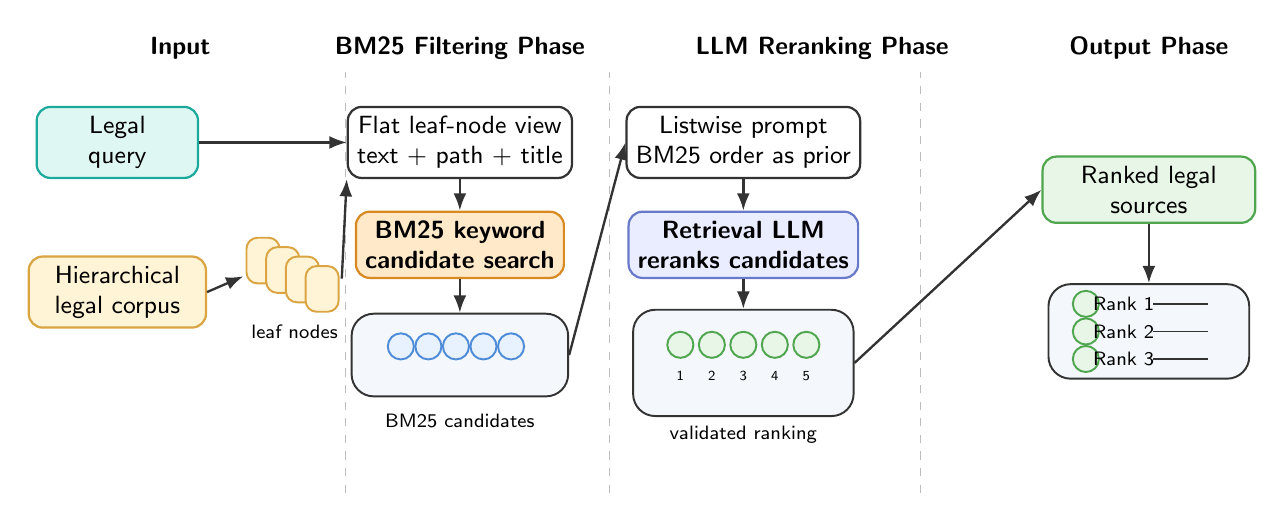
\begin{tikzpicture}

% Phase labels.
\node[phase] at (1.1,5.65) {Input};
\node[phase] at (4.65,5.65) {BM25 Filtering Phase};
\node[phase] at (9.25,5.65) {LLM Reranking Phase};
\node[phase] at (13.4,5.65) {Output Phase};

% Input.
\node[query] (query) at (0.3,4.45) {Legal\\query};
\node[corpus] (corpus) at (0.3,2.55) {Hierarchical\\legal corpus};

% Corpus icon stack.
\foreach \x/\y in {2.15/2.95,2.4/2.83,2.65/2.71,2.9/2.59} {
  \node[doc] at (\x,\y) {};
}
\node[font=\scriptsize] at (2.55,2.05) {leaf nodes};

% BM25 filtering.
\node[artifact] (flat) at (4.65,4.45) {Flat leaf-node view\\text + path + title};
\node[bm25] (bm25) at (4.65,3.15) {BM25 keyword\\candidate search};

\node[softbox, minimum width=2.75cm, minimum height=1.05cm] (candidatebox) at (4.65,1.75) {};
\foreach \x in {3.9,4.25,4.6,4.95,5.3} {
  \node[node] at (\x,1.86) {};
}
\node[font=\scriptsize] at (4.65,0.92) {BM25 candidates};

% LLM reranking.
\node[artifact] (rerankprompt) at (8.25,4.45) {Listwise prompt\\BM25 order as prior};
\node[llm] (reranker) at (8.25,3.15) {Retrieval LLM\\reranks candidates};

\node[softbox, minimum width=2.8cm, minimum height=1.35cm] (rerankedbox) at (8.25,1.65) {};
\foreach \x/\lab in {7.45/1,7.85/2,8.25/3,8.65/4,9.05/5} {
  \node[finalnode] at (\x,1.88) {};
  \node[font=\tiny] at (\x,1.48) {\lab};
}
\node[font=\scriptsize] at (8.25,0.74) {validated ranking};

% Output.
\node[output] (ranked) at (13.4,3.85) {Ranked legal\\sources};
\node[softbox, minimum width=2.55cm, minimum height=1.2cm] (rankbox) at (13.4,2.05) {};
\foreach \y/\lab in {2.4/1,2.05/2,1.7/3} {
  \node[finalnode] at (12.6,\y) {};
  \node[font=\scriptsize] at (13.08,\y) {Rank \lab};
  \draw[darkline, line width=0.5pt] (13.45,\y) -- (14.15,\y);
}

% Main flow.
\draw[flow] (query.east) -- (flat.west);
\draw[flow] (corpus.east) -- (1.9,2.75);
\draw[flow] (3.15,2.72) -- (flat.south west);
\draw[flow] (flat) -- (bm25);
\draw[flow] (bm25) -- (candidatebox);
\draw[flow] (candidatebox.east) -- (rerankprompt.west);
\draw[flow] (rerankprompt) -- (reranker);
\draw[flow] (reranker) -- (rerankedbox);
\draw[flow] (rerankedbox.east) -- (ranked.west);
\draw[flow] (ranked) -- (rankbox);

% Phase separators.
\draw[faint] (3.2,0.0) -- (3.2,5.35);
\draw[faint] (6.55,0.0) -- (6.55,5.35);
\draw[faint] (10.5,0.0) -- (10.5,5.35);

\end{tikzpicture}
\end{document}
